\section{Methods}
\label{sec:methods}
We lay a foundation for quantitative conflict analysis of multi-objective systems. The analysis centers on the use of three metrics: two existing measures from EMO and one that we have developed and introduce for the first time here. A case study on the impacts of climate change on forest management serves to illustrate the conflict analysis. Prior to describing the case study, we first define terminology and describe each of the measures used in our analysis.

\subsection{Terminology}
\label{subsec:terminology}
  
\paragraph{The multi-objective problem}
Consider the $M$-objective optimization problem
\begin{align}
\text{Maximize}& \notag \\
& \mathbf{f} = [f_1(\mathbf{x}), f_2(\mathbf{x}), \ldots, f_M(\mathbf{x}) ] \label{eqn:generalObj}\\
\text{subject to}& \notag \\
& \mathbf{x} \in X \label{eqn:generalConstraint}
\end{align}
with \textit{objective functions} $f_i(\mathbf{x}), i \in \{1,\ldots,M\}$ and feasible \textit{decision vectors} (or \textit{solutions}) $\mathbf{x} \in \mathbb{R}^n$ where $n$ is the number of decision variables in the optimization problem. A set of equality and inequality constraints determine the \textit{feasible decision space} $X$. Solutions in $X$ are referenced by superscripts: $X = \{\mathbf{x}^1,\mathbf{x}^2,\ldots,\mathbf{x}^{|X|}\}$. Each objective function $f_i : \mathbb{R}^n \mapsto \mathbb{R}$ maps decision vectors to scalars in $\mathbb{R}$. The vector objective function $\mathbf{f} : X \mapsto \mathbb{R}^M$ maps the feasible decision space to the \textit{objective space} $\mathbb{R}^M$. The set of all objective functions is the \textit{objective set} $\mathcal{M} = \{f_1,\ldots,f_M\}$.

\paragraph{Dominance and frontiers}
A solution $\mathbf{x}^1$ is said to \textit{dominate} another solution $\mathbf{x}^2$ ($\mathbf{x}^1 \succ \mathbf{x}^2$) if
\begin{align}
\exists f_i \in \mathcal{M} : f_i(\mathbf{x}^1) > f_i(\mathbf{x}^2) \text{ and } \forall f_i \in \mathcal{M} \; f_i(\mathbf{x}^1) \ge f_i(\mathbf{x}^2)
\end{align}
A solution $\mathbf{x}^1 \in X$ is \textit{non-dominated} if
\begin{align}
\nexists \mathbf{x}^2 \in X : \mathbf{x}^2 \succ \mathbf{x}^1
\end{align}
For a rational decision maker, all dominated solutions may be removed from the analysis, since for a dominated solution $\mathbf{x}^2$ there exists another solution $\mathbf{x}^1$ which is better: $\mathbf{x}^1$ achieves more in at least one objective than $\mathbf{x}^2$, and $\mathbf{x}^1$ does not achieve less in any objective than $\mathbf{x}^2$. Thus, the decision maker will always select a solution from the set of non-dominated decision vectors that solve the multi-objective problem \eqref{eqn:generalObj} and \eqref{eqn:generalConstraint}. We refer to this set as the \textit{Pareto-optimal set} $P = \{\mathbf{x} \in X | \nexists \mathbf{y} \in X : \mathbf{y} \succ \mathbf{x} \}$.

The \textit{Pareto-optimal frontier}, the \textit{efficient frontier} or, simply, the \textit{frontier} $Z$ is the corresponding set of $M$-dimensional \textit{objective vectors} $\mathbf{z} = [f_1(\mathbf{x}),f_2(\mathbf{x}),\ldots,f_M(\mathbf{x})]$. That is,
\begin{align}
Z = \{\mathbf{z} = [f_1(\mathbf{x}),\ldots,f_M(\mathbf{x})] \:|\: \mathbf{x} \in P\}
\end{align}
Objective vectors' components are referred to in subscripts:
\begin{align}
\mathbf{z} = [z_1, z_2, \ldots, z_M]
\end{align}
Objective vectors provide the decision maker with knowledge of the objective achievement of a solution $\mathbf{x}$ - the $i$th component of an objective vector $\mathbf{z}$ represents the achievement in objective $i$ by the corresponding decision vector $\mathbf{x}$.

\paragraph{Ideal and nadir objective vectors}
The \textit{ideal objective vector} is defined as the vector
\begin{align}
\mathbf{z}^{\text{ideal}} = \max_{\mathbf{x} \in X}\{f_i(\mathbf{x})\} \quad \forall i \in \mathcal{M}.
\end{align}
Analogously, define the nadir solution as the vector
\begin{align}
\mathbf{z}^{\text{nadir}} = \min_{\mathbf{x} \in X}\{f_i(\mathbf{x})\} \quad \forall i \in \mathcal{M}.
\end{align}
The ideal objective vector represents the impossible ideal scenario in which each objective is simultaneously optimized. The nadir objective vector represents the worst case scenario in which each objective attains its lowest value. These solutions are the diagonal corners of the minimum bounding box for the efficient frontier $Z$. Since they provide upper and lower bounds for each objective, they serve as reference points against which the decision maker can compare solutions. 

\paragraph{Trade-offs}
The \textit{trade-off} between two objective vectors $\mathbf{z}^1$ and $\mathbf{z}^2$ is the vector of differences in their objective achievements:
\begin{align}
\mathbf{\tau}^{1,2} = [z^2_1 - z^1_1, z^2_2 - z^1_2, \ldots, z^2_M - z^1_M]
\end{align}
The components of $\mathbf{\tau}^{1,2}$ represent the amount of each objective that would be sacrificed or gained by selecting $\mathbf{z}^2$ instead of $\mathbf{z}^1$.
Note that $\mathbf{\tau}^{1,2} = - \mathbf{\tau}^{2,1}$. 

\paragraph{Sub-dimensions}
During analysis, we often wish to consider only a subset of the objectives $\mathcal{L} \subset\mathcal{M}$. We define such subsets as \textit{sub-dimensional objective sets}. In these cases, it is simpler to work with constructs that have only those components that correspond to the objectives in $\mathcal{L}$. For instance, define the \textit{sub-dimensional objective vector} for the solution $\mathbf{x}^i$ as $\mathbf{z}^i_\mathcal{L}$ which has components $\forall \ell \in \mathcal{L}. \, z^i_\ell = f_\ell(\mathbf{x}^i)$.
Define the \textit{sub-dimensional trade-off} $\tau^{1,2}_\mathcal{L}$ as the vector with components $\forall \ell \in \mathcal{L}. \, \tau^{1,2}_\ell$.

\paragraph{Relative objective achievements, relative objective vectors, and relative trade-offs}
Using the nadir and ideal objective vectors, we can represent each solution as a vector of its relative objective achievements. This allows for dimensionless and scale-agnostic comparison of solutions. For an objective vector $\mathbf{z}$, its \textit{relative achievement in objective} $i$ is
\begin{align}
\overbar{z_i} = \frac{z_i - z^\text{nadir}_i}{z^\text{ideal}_i - z^\text{nadir}_i},
\end{align}
and the corresponding \textit{relative objective vector} is
\begin{align}
\overbar{\mathbf{z}} = [\overbar{z_1},\overbar{z_2},\ldots,\overbar{z_M}].
\end{align}
For two objective vectors $\mathbf{z}^1$ and $\mathbf{z}^2$, the corresponding \textit{relative trade-off} is
\begin{align}
\overbar{\mathbf{\tau}}^{1,2} = \left[\overbar{z^2_1} - \overbar{z^1_1}, \overbar{z^2_2} - \overbar{z^1_2}, \ldots, \overbar{z^2_M} - \overbar{z^1_M}\right]
\end{align}

\paragraph{Conflict, monotonicity, bundles and stacks}
We use the following test to determine if Objectives in an objective set $\mathcal{L}$ \textit{do not conflict} if the objectives improve simultaneously:
$\forall \mathbf{z}^1, \mathbf{z}^2 \in Z, i \in \mathcal{L}$
\begin{align}
(z^1_i \ge z^2_i) \Rightarrow (z^1_j \ge z^2_j) \quad \forall j \in \mathcal{L}, j \neq i \label{eqn:objPairHarmony}
\end{align}
If \eqref{eqn:objPairHarmony} does not hold, then the objectives conflict. Any pair of objectives $i,j \in \mathcal{M}$ such that equation \eqref{eqn:objPairHarmony} holds are said to \textit{increase monotonically}. In the case of monotonically increasing objectives $i$ and $j$, improving objective $i$ also yields improvement in objective $j$. Conversely, if 
\begin{align}
(z^1_i \ge z^2_i) \Rightarrow (z^1_j \le z^2_j) \quad \forall \mathbf{z}^1, \mathbf{z}^2 \in Z, j \neq i \label{eqn:objPairMonoDec}
\end{align}
holds, then objectives $i$ and $j$ are said to \textit{decrease monotonically}.

When the objectives represent goods or services, a set of objectives that conflict is defined as a \textit{bundle} and a set of objectives that do not conflict is defined as a \textit{stack}.

Equation \eqref{eqn:objPairHarmony} checks for monotonically increasing relationships among objectives. This means of detecting conflict is functionally equivalent to that used by many studies, such as Brockhoff and Zitzler (2009) \cite{brockhoff2009objective} and Purshouse and Fleming (2003) \cite{purshouse2003conflict}.

\subsection{Measuring conflict: the hypervolume indicators}
\label{sec:waysToMeasureFrontiers}
% given a system, here's what we're going to measure and how we'll measure it.
Any multi-objective problem whose efficient frontier consists of more than one solution contains conflict. The decision maker responsible for these multi-objective systems must determine which solution represents the best compromise among the objectives, and their ability to do so is improved by knowledge of the conflict in the system. This includes both the amount of overall system conflict as well as the source of that conflict. For the former, we can draw on existing measures from EMO; for the latter, we propose a new metric that quantifies the conflict between pairs of objectives. We begin with a description of the measures from EMO that we use to measure system-level conflict: the hypervolume indicators.

\subsubsection{Hypervolume indicator}
The \textit{hypervolume indicator} $I_{H1}(Z)$ measures the percentage of the objective space that is bounded by the non-dominated objective vectors $\mathbf{z} \in Z$. See Figure \ref{fig:frontierVolumes}. Systems with less conflict will produce solutions with greater joint provision of objectives, leading to a greater proportion of enclosed objective space and thus a larger value for the hypervolume. In contrast, systems with more conflict produce solutions with less joint provision of objectives, leading to a lesser proportion of enclosed objective space and a smaller value for the hypervolume. That is, the greater the value of the hypervolume indicator, the lower the conflict in the system.

\begin{figure}[ht]
\centering
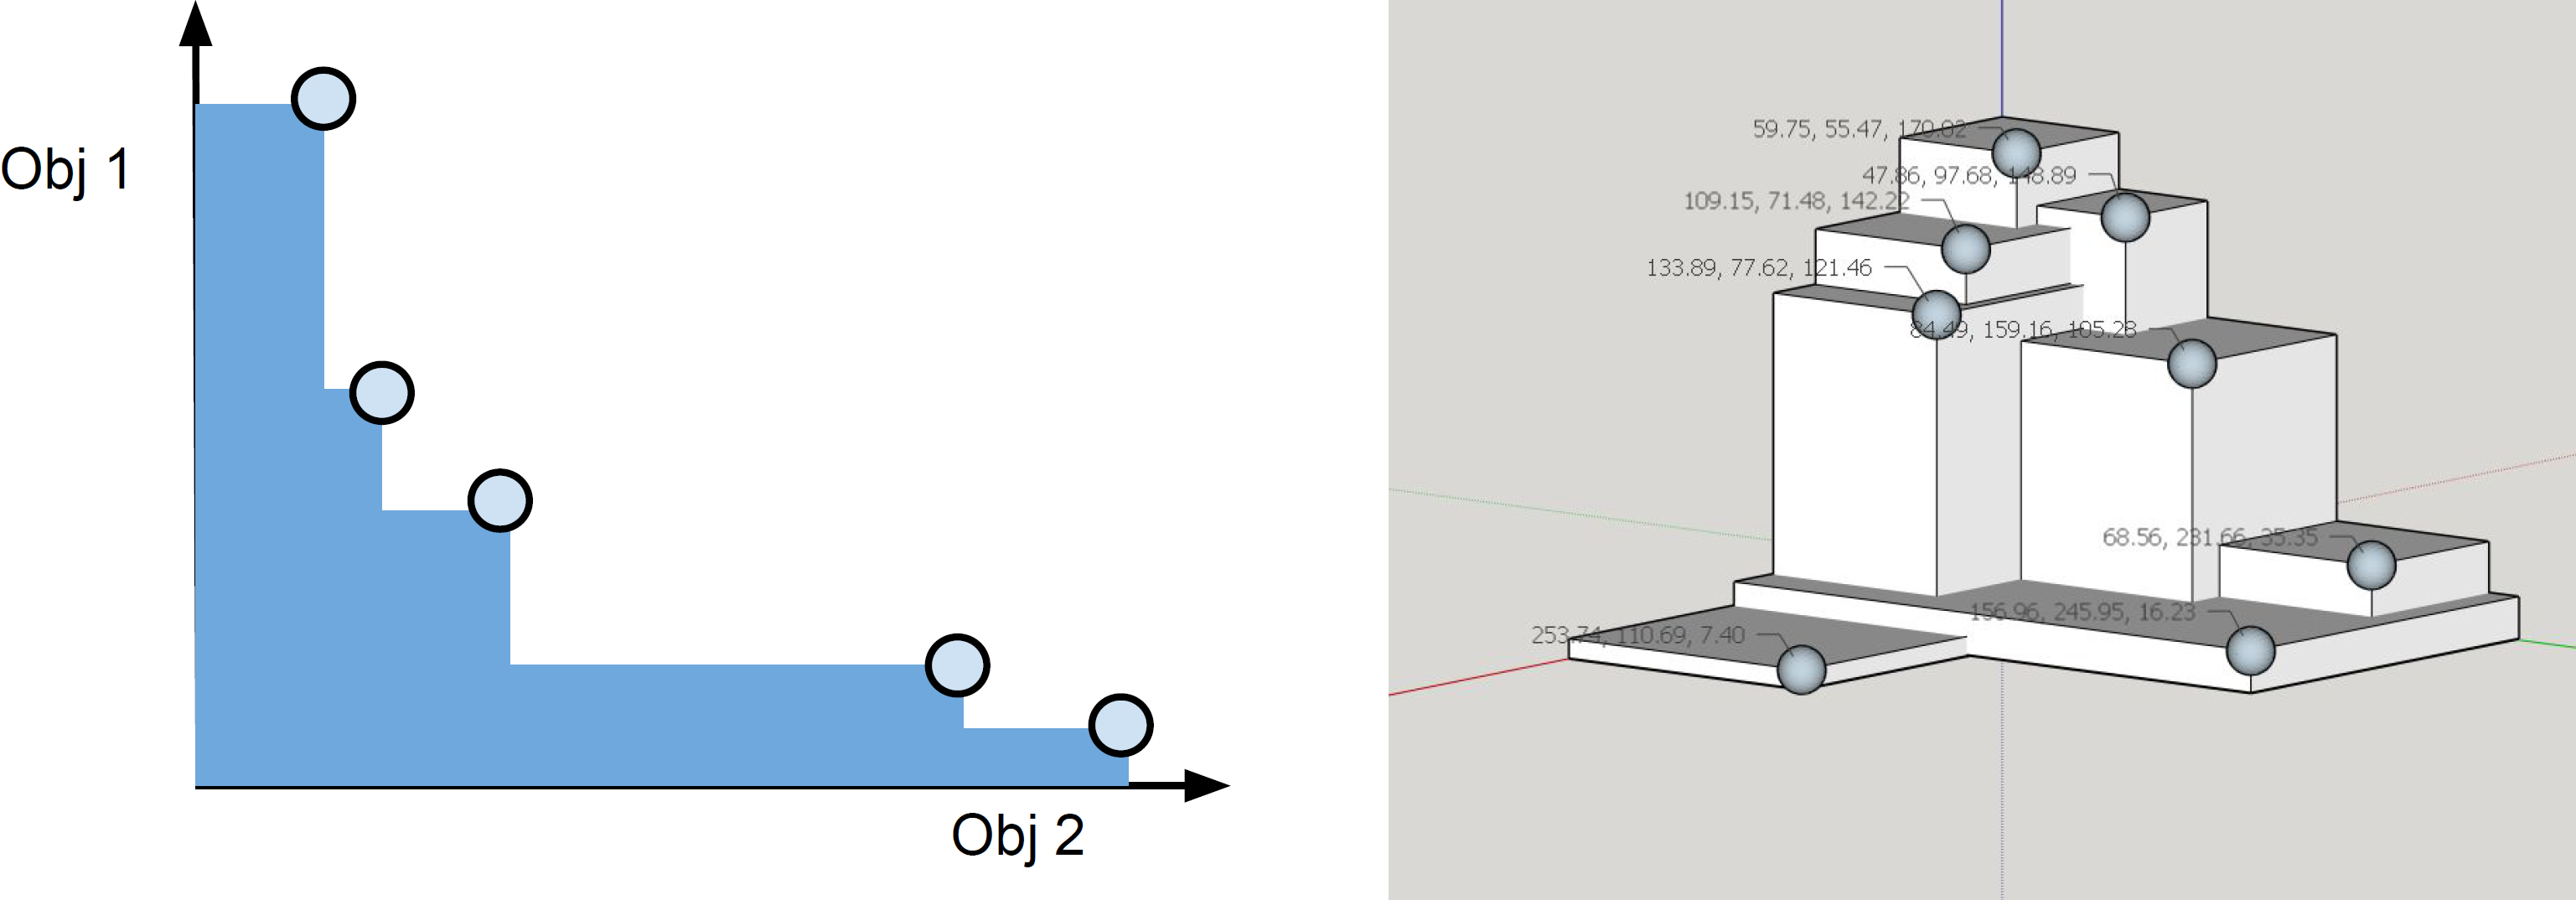
\includegraphics[width=.85\textwidth]{../images/FrontierVolumesNo2DOutlines}
\caption[Hypervolume of Pareto frontiers]{Depiction of the hypervolumes of frontiers with two objectives (left) and three objectives (right).}
\label{fig:frontierVolumes}
\end{figure}

To measure the hypervolume indicator, for each relative objective vector $\overbar{\mathbf{z}^i}$ in the frontier $Z$, define its corresponding hyperrectangle $r_i$. $r_i$ is the $M$-orthotope with the pair of diagonally opposite points the origin and the point defined by the components of the relative objective vector $\overbar{\mathbf{z}^i}$. Then the hypervolume indicator is the volume of the union of these hyperrectangles:
\begin{align}
I_{H1}(Z) = \text{vol} \left( \bigcup_{i = 1}^{|Z|} r_i \right). \label{eqn:hypervol}
\end{align}
Given two frontiers $Z^1$ and $Z^2$, how do you interpret a difference in their hypervolumes? Consider Figure \ref{fig:Hypervol10percent} which shows the relative objective space for a two-dimensional frontier. The shaded square in the lower left represents an achievement of 10\% in each objective. Since the objective space of the relative objective vectors is bounded by the $1 \times 1$ square, this corresponds to 1\% of the objective space. So if $Z^1$ and $Z^2$ are bi-objective frontiers ($M=2$) and if $I_{H1}(Z^1) - I_{H1}(Z^2) = 0.01$, then the solutions in frontier $Z^1$ bound an area equivalent to an additional 10\% achievement in each objective beyond that bounded by the solutions in $Z^2$. Small differences in the values of the hypervolume represent significant objective gains.

In general, an increase of $h$ in the value of the hypervolume equates to an increase in each objective of $h^{1/M}$. So if $Z^1$ and $Z^2$ were tri-objective ($M=3$) then an improvement of $.01$ in the value of the hypervolume would represent an improvement of about 22\% in each objective.

\begin{figure}
\centering

\includegraphics[width=.5\textwidth]{../images/HypervolumeImprovements}
\caption[Interpreting differences in hypervolumes]{To compute the hypervolume, we use the relative objective vectors for the solutions in a frontier. As a result, the frontier is bounded by the $M$-cube which has a pair of diagonal corners at the origin and $\vec{1}$. Shown here is the 2-cube (a square) representing the space in which we compute the hypervolume for a bi-objective frontier ($M=2$). The space bound by the shaded square in the lower left represents an achievement of 10\% in each objective yet makes up only 1\% of the objective space. Its intent is to show that small differences in hypervolumes are significant: with two objectives, an improvement of 0.01 in the value of the hypervolume represents an additional achievement of 10\% in each objective.}
\label{fig:Hypervol10percent}
\end{figure}

\subsubsection{Binary Hypervolume Indicator}
If a frontier $Z^2$ is found to have a smaller hypervolume than another $Z^1$, one may wonder whether $Z^2$ is completely enclosed within $Z^1$ or simply bounds a different but smaller region of the relative objective space. We use the binary hypervolume indicator to address this question. The binary hypervolume $I_{H2}(Z^1,Z^2)$ computes the volume of the objective space bounded by $Z^1$ but not by $Z^2$. See Figure \ref{fig:binaryHypervolume}. As such, if $Z^2$ is completely enclosed within $Z^1$, then $I_{H2}(Z^2,Z^1) \le 0$. On the other hand, if $I_{H2}(Z^2,Z^1) > 0$ then $Z^2$ encloses regions of the objective space that $Z^1$ does not.

Following the definition proposed by Zitzler (1999) \cite{zitzler1999evolutionary}, the \textit{binary hypervolume indicator} of two frontiers $Z^1$ and $Z^2$ is \cite{zitzler1999evolutionary}
\begin{align}
I_{H2} (Z^1,Z^2) = I_{H1} (Z^1 + Z^2) - I_{H1} (Z^2)
\end{align}
where $I_{H1} (Z^1 + Z^2)$ is the unary hypervolume indicator of the frontier that consists of the nondominated points in $\{Z^1 \cup Z^2\}$. See the lower-left panel in Figure \ref{fig:binaryHypervolume}.

\begin{figure}[ht]
\centering
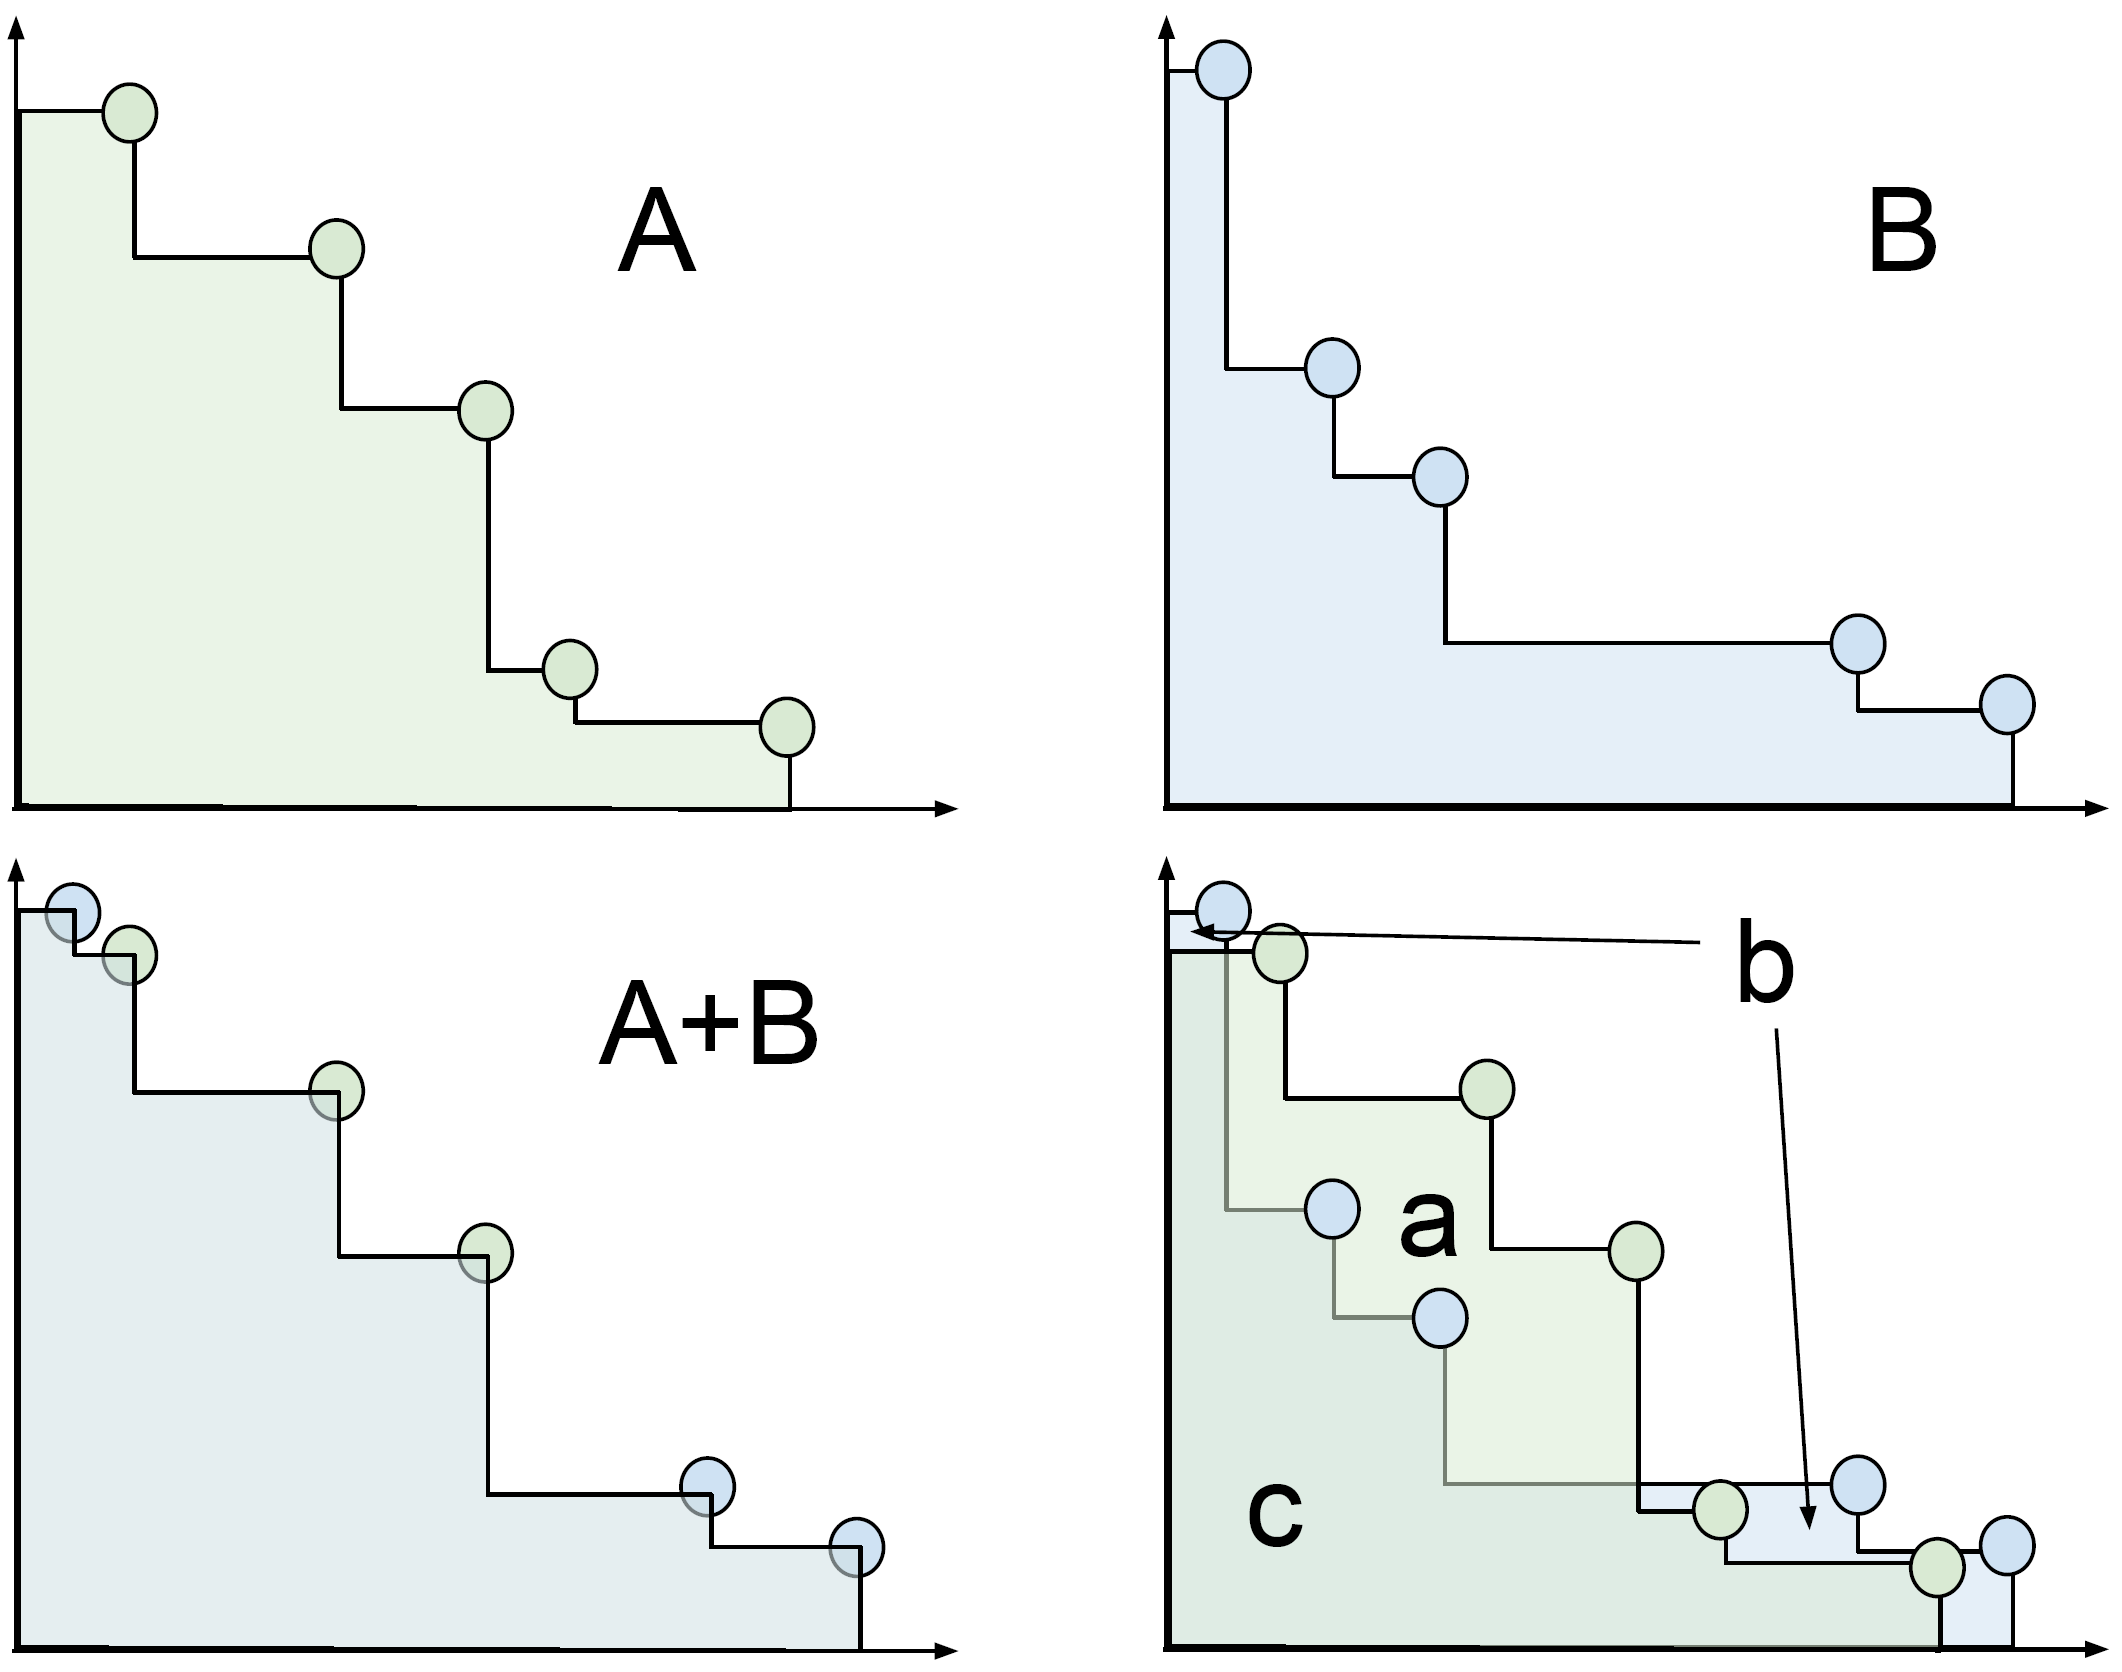
\includegraphics[width=.7\textwidth]{../images/BinaryHypervolume}
\caption[Binary hypervolume indicator]{Depiction of the binary hypervolume indicator. The individual frontiers are shown in the top row: frontier $A$ (left) and frontier $B$ (right). The merged frontier $A+B$ is shown in bottom left - note the absence of points that were dominated when combined. Following the naming of regions as shown in the bottom right figure, the binary hypervolume indicator is equal to
\begin{minipage}{\linewidth}
  \begin{align*}
    I_{H2} (A,B) = \left(\text{area}_a + \text{area}_b + \text{area}_c \right) - \left( \text{area}_b + \text{area}_c \right) = \text{area}_a
  \end{align*}
\end{minipage}%
}
\label{fig:binaryHypervolume}
\end{figure}

\subsection{Computing the hypervolume indicator}
Computing the hypervolume is a nontrivial task that has received attention from the EMO community. For a comparison of previous algorithms that compute the hypervolume, see While (2006) \cite{while2006faster}. For this work, we developed our own algorithm to compute the hypervolume indicator.

The algorithm begins with a list of the relative objective vectors, denoted in the algorithm simply by $\mathbf{z} \in Z$. These vectors are assumed to be sorted in descending order based on their $m$th component, for some arbitrary objective $m \in \mathcal{M}$. We define the sub-dimensional objective set $\mathcal{L} = \mathcal{M} \backslash \{m\}$ whose cardinality we denote by $|\mathcal{L}| = L = M - 1$.

We initialize the algorithm with an empty set of non-dominated solutions in $L$ dimensions; refer to this set as $G$. Let the volume of this nondominated set be denoted $\overbar{V}$. We sequentially add solutions from $Z$ to $G$, at each iteration adding the contribution of the solution $\mathbf{z}$ to the hypervolume indicator $V$. These contributions are computed by multiplying the solution's $m$th component $z_m$ by its contribution to the volume of $G$, $\overbar{V}_\mathbf{z}$. See Figure \ref{fig:AlgoAid} for a visual reference (the solutions' contribution to the volume of $G$, $\overbar{V}_\mathbf{z}$, are the yellow regions in the figure).

$\overbar{V}_\mathbf{z}$ is computed as follows. Initialize $\overbar{V}_\mathbf{z} = 0$, and add $\mathbf{z}$ to the set $G$. Remove from $G$ any solutions that are dominated by $\mathbf{z}$ in $L$ dimensions. Add to $\overbar{V}_\mathbf{z}$ the value of the volume of $\mathbf{z}$ in $L$ dimensions (the union of the yellow and gray areas in Figure \ref{fig:AlgoAid}); this is simply the product of its components $z_\ell$ for $\ell \in \mathcal{L}$. Then subtract from $\overbar{V}_\mathbf{z}$ the volume of $G$ prior to the addition of $\mathbf{z}$ (the union of the gray and white areas in Figure \ref{fig:AlgoAid}). The last step is to compute and add back in the volume of the ``sides'' of $G$ that were subtracted in the previous step (the white areas in Figure \ref{fig:AlgoAid}). This volume is computed by taking the sum over each dimension $\ell \in \mathcal{L}$ of the areas along that dimension enclosed by the existing solutions in $G$. Pseudocode for this algorithm is presented in Figure \ref{algo:HypervolAlgo}.

\newpage
\begin{figure}[H]
\caption[Algorithm to compute the hypervolume indicator of a Pareto frontier]{Algorithm to compute the hypervolume $V$ of a Pareto frontier. Prior to running the algorithm, pick an objective $m$ from the objective set $\mathcal{M}$ and define the sub-dimensional objective set $\mathcal{L} = \mathcal{M} \backslash \{m\}$. Then sort $\mathbf{z} \in Z$ in descending order by their $m$th component. Here, $\mathbf{z} \in Z$ is the set of relative objective vectors. Let $\overbar{V_\mathbf{z}}$ be the ($M-1$)-dimensional volume contribution of the solution $\mathbf{z}$, and let $\mathbf{g} \in G$ be the non-dominated objective vectors in $M-1$ dimensions.}
\label{algo:HypervolAlgo}
\begin{algorithmic}[1]

\State $V \gets 0$
\State $\overbar{V} \gets 0$
\State $G \gets \emptyset$

% Iterate over each solution
\ForAll{$\mathbf{z} \in Z$}

	\State $\overbar{V}_\mathbf{z} \gets \prod_{\ell \in \mathcal{L}} z_\ell - \overbar{V}$
		
	\ForAll{$\mathbf{g} \in G$}
		\If{$g_\ell < z_\ell \, \forall \ell \in \mathcal{L}$}
			\State $G \gets G \backslash \{\mathbf{g}\}$
		\EndIf
	\EndFor
	
	% iterate over subdimensions to "add back the sides"	
	\ForAll{$\ell \in \mathcal{L}$}
	
		\State $G_{\mathbf{z},\ell} := \set{\mathbf{g} \in G : g_\ell > z_\ell}$
		
		\State Sort $\mathbf{g} \in G_{\mathbf{z},\ell}$ in ascending order by $\ell$th component, $g_\ell$
		
		\State $v_i \gets z_\ell$
		\ForAll{$\mathbf{g} \in G_{\mathbf{z},\ell}$}
			\State $v_t \gets g_\ell$
			\State $\delta_\ell := v_t - v_i$
			\State $\overbar{V}_\mathbf{z} \gets \overbar{V}_\mathbf{z} + \delta_\ell \prod_{\lambda \in \mathcal{L} \backslash \{\ell\}} g_\lambda$
			\State $v_i \gets v_t$
		\EndFor
		
	\EndFor
	
	\State $G \gets G \cup \{\mathbf{z}\}$
	\State $\overbar{V} \gets \overbar{V} + \overbar{V}_\mathbf{z}$
	\State $V \gets V + z_m \overbar{V}_\mathbf{z}$
\EndFor


\end{algorithmic}
\end{figure}

\begin{figure}[ht]
\centering
\caption[First iterations for computing $\overbar{V}$]{\textbf{Computing the hypervolume of a 3D frontier: first three iterations of the algorithm}. Consider a three-dimensional frontier $Z$. We sequentially add solutions to a 2D projection of the frontier, seen here (process moves from left to right). The solutions are added in order of decreasing value in their third component (height -- not seen here). At each iteration, we compute the contribution in 2D as follows: Add the product of the solution's 2D components (the union of the yellow and gray areas). Then subtract all the previous existing frontier area (the union of the gray and white areas). Then add back the value of the sides (white areas). This yields the value of the yellow area. Multiply this value by the third component of the solution to obtain the solution's contribution to the hypervolume $V$.}
\label{fig:AlgoAid}
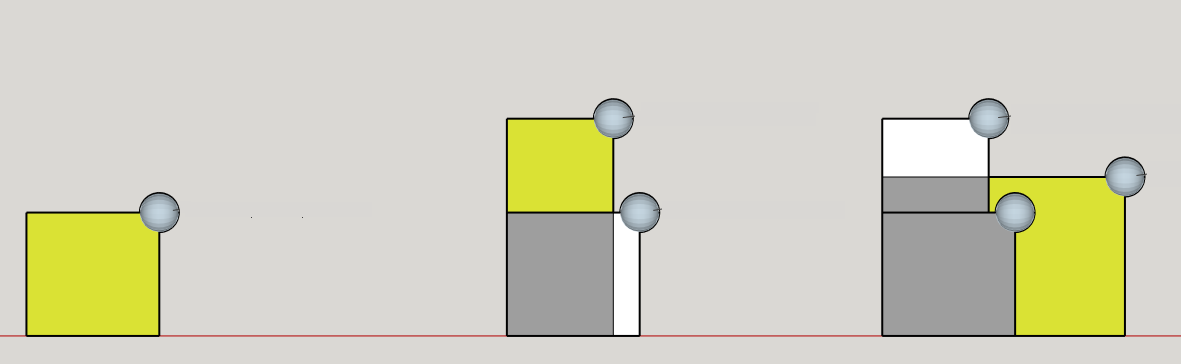
\includegraphics[width=.85\textwidth]{../images/3DFrontierSchematic_SketchUp_FirstSteps_2D_clean}
\end{figure}

\subsection{A new measure for pairwise objective conflict}
\label{sec:newConflictMetric}
% This is our cool new way of drilling down into an objective pair to assess conflict
When the hypervolume indicates that there is conflict in the system, how does the decision maker determine which objectives are responsible for the conflict? In the case of the hospital, is it cost and patient throughput that are most conflicting, or is it cost and required back-up? For the forest manager, are carbon sequestration and timber revenue the incompatible objectives responsible for the low hypervolume value, or is it wildlife habitat and timber revenue? If the forest manager oversees multiple independent forests, they may also ask whether the answers to these questions are the same in each. With the suite of measures currently available, the decision maker cannot adequately answer these questions. Here we propose a new measure of conflict to fill the void.

Consider the frontiers in Figure \ref{fig:ConflictVariesExample}. The conflict between maximization objectives $i$ and $j$ is greatest in Frontier C and least in Frontier A.
\begin{figure}[ht]
\centering

\includegraphics[width=.6\textwidth]{../images/ConflictVariesExample}
\caption[Example of varying conflict between objectives]{Varying conflict between objectives. The conflict between maximization objectives $i$ and $j$ increases from Frontier A to Frontier B to Frontier C.}
\label{fig:ConflictVariesExample}
\end{figure}

Many authors have previously measured conflict between objectives \cite{brockhoff2009objective}\cite{purshouse2003conflict}\cite{gal1977redundant}, with most commonly used metrics deriving from measures of linear correlation (such as the Pearson correlation coefficient \cite{deb2006searching}) or rank correlation (such as Kendall's Tau \cite{kanoulas2009empirical} or Spearman's rho \cite{karande2012application}). The motivation behind these metrics is often the removal of redundant objectives from a many-objective optimization problem. In such cases, measures of monotonicity or correlation alone suffice. However, the current metrics fall short of providing a quantification of conflict between pairs of objectives. Metrics for linear correlation are limited in their ability to capture the montonicity between objectives, which is the fundamental principle that determines if objectives conflict. Furthermore, both linear and rank correlation metrics fail to capture the objective achievement of the solutions. Thus, for a more nuanced understanding of the relationship between the objectives, a different metric is required.

Let $\mathbf{z}_{ij}$ be the sub-dimensional objective vector comprised of only the components corresponding to the $i$th and $j$th objectives $\mathbf{z}_{ij} = [z_i,z_j]$. We define the following measure of conflict between objectives $i$ and $j$:
\begin{align}
C_{ij} = \frac{(1-\rho_{ij})\overbar{d}_{ij}}{2 d_{\max,ij}} \label{eqn:defConflict}
\end{align}
where $\overbar{d}_{ij}$ is the average sub-dimensional distance from objective vectors to the ideal solution:
\begin{align}
\overbar{d}_{ij} = \frac{1}{|Z|} \sum_{\mathbf{z} \in Z} ||\mathbf{z}^{\text{ideal}}_{ij} - \mathbf{z}_{ij}||
\end{align}
and
\begin{align}
d_{\max,ij} = ||\mathbf{z}^{\text{ideal}}_{ij} - \mathbf{z}^{\text{nadir}}_{ij}||
\end{align}
and $\rho_{ij}$ is Spearman's rank-correlation coefficient for the solutions' achievements in objectives $i$ and $j$. Note that $C_{ij} \in [0,1)$, taking smaller values when there is less conflict between objectives $i$ and $j$ and larger values when there is more.

The conflict metric proposed here (equation \eqref{eqn:defConflict}) addresses two major issues:
\begin{enumerate}
\item \textbf{Indifference to non-conflicting relationships}. Per equation \eqref{eqn:objPairHarmony}, when an objective $i$ increases monotonically with another objective $j$, the objectives do not conflict. Accordingly, $C_{ij}$ should equal 0 in all such cases. This is true for the new metric, since for monotonically increasing objectives $\rho_{ij} = 1$, so $1-\rho_{ij} = 0$.
\item \textbf{Consideration of objective achievement}. Recall Figure \ref{fig:ConflictVariesExample} and the intuitive notion that the conflict between objectives $i$ and $j$ is stronger in Frontier C than it is in Frontier B than it is in Frontier A. This notion is guided by the idea that the closer objective vectors are to the sub-dimensional ideal solution on average, the less the conflict between the objectives; that is, that greater simultaneous objective provision is indicative of less conflict. The proposed metric accounts for this, while correlation measures do not. In the extreme case of monotonically decreasing objectives, $\frac{(1-\rho_{ij})}{2} = 1$, so $C_{ij} = \frac{\overbar{d}{ij}}{d_{\max,ij}}$. See Figure \ref{fig:WhyOursIsBetter} for an example.
\end{enumerate}
\begin{figure}[ht]
\centering

\includegraphics[width=.9\textwidth]{../images/WhyOursIsBetter}
\caption[Comparing the proposed conflict metric to others used in multi-objective optimization]{Comparing the proposed metric for conflict $C_{ij}$ against the Pearson product-moment and the Spearman rank correlation coefficients ($\rho_{ij}$ and $\rho_{s,ij}$, respectively). While the latter two are identical for frontiers A and C, the proposed metric is greater for frontier C than it is for A. This is because it accounts for the average relative distance to the sub-dimensional ideal objective vector.}
\label{fig:WhyOursIsBetter}
\end{figure}

To interpret differences in $C_{ij}$ for different objective pairs, we decompose the metric into components: one for rank correlation
\begin{align}
c_{ij,\rho} = \frac{1-\rho_{ij}}{2},
\end{align}
and one for objective achievement
\begin{align}
c_{ij,d} = \frac{\overbar{d}{ij}}{d_{\max,ij}}.
\end{align}
The components for different objective pairs ($i,j$) can be used to determine whether the 

%=====

\subsection{Case Study}
\label{sec:caseStudy}
To demonstrate the application of the hypervolume indicators and the proposed pairwise objective metric to the analysis of conflict in multi-objective systems, we perform a case study on forest management in the Deschutes National Forest. We compare the conflict among ecosystem services in three multi-objective systems: one in which climate change is ignored, one in which climate change is predicted to be mild, and one in which it is predicted to be severe. For each climate change scenario, we solve a multi-objective mathematical program that optimizes ecosystem service achievement. Specifically, the model aims to minimize fire hazard and sediment delivery while maximizing habitat for the northern spotted owl. In the coming sections we describe the study area and the importance of each of these ecosystem services. We then formally define the mathematical program solved for each climate change scenario and describe the climate scenarios considered.

\subsubsection{Study area and selection of ecosystem services}
\label{subsec:studyArea}
To appreciate the selection of the ecosystem services, we first describe the area in which the case study was conducted. The area is known as the Drink Planning Area. It consists of 7056 ha of federally owned forest land on the east slopes of the Cascade Mountain Range located within the Deschutes National Forest. See Figure \ref{fig:drinkOverview}. The Drink contains large areas of old growth forest, having not been logged for many years. The large swaths of old growth forest in the Drink make it prime habitat for the northern spotted owl (NSO) (\textit{Strix occidentalis caurina}, Figure \ref{fig:nso}), an iconic % (albeit controversial \cite{simberloff1998flagships}) 
inhabitant of Pacific Northwest forests that is listed as a federally threatened species \cite{congress1973endangered}. However, the same old growth conditions that render the area suitable habitat for the NSO also render it susceptible to high-severity wildfires. Such a wildfire would put at risk the NSO's habitat \cite{courtney2004scientific} as well as one of the Drink's other notable features - the municipal watershed for the cities of Bend, OR and Sisters, OR. Wildfires pose a threat to the cities' water supply, because they can cause soil water repellency, surface runoff, and debris torrents \cite{ice2004effects} which degrade watershed quality.

\begin{figure}[ht]
\centering
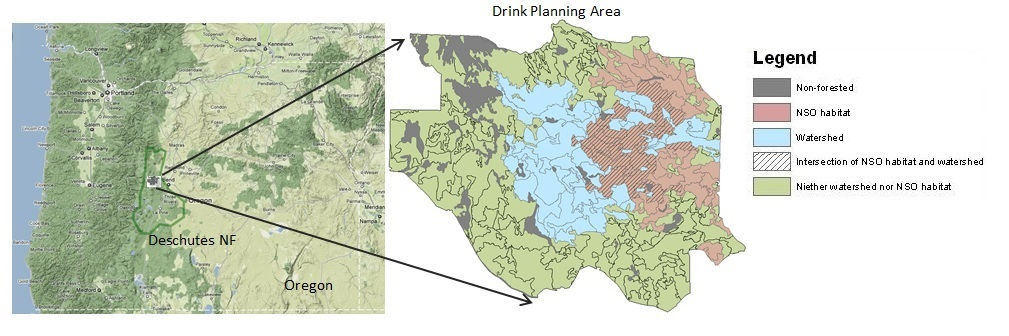
\includegraphics[width=.9\textwidth]{../images/Drink_Overview}
\caption[Overview of the study system, the Drink Planning Area]{Overview of the study system, the Drink Planning Area, consisting of 7056 ha in the Deschutes National Forest. The Drink Area contains old growth forest that make it suitable habitat for the northern spotted owl. It also houses the municipal watershed for Bend, OR and Sisters, OR.}
\label{fig:drinkOverview}
\end{figure}

\begin{figure}
\centering
\caption[Northern spotted owl]{The northern spotted owl is a threatened species whose habitat includes forests in the Pacific Northwest, including the Drink Area.}
\label{fig:nso}
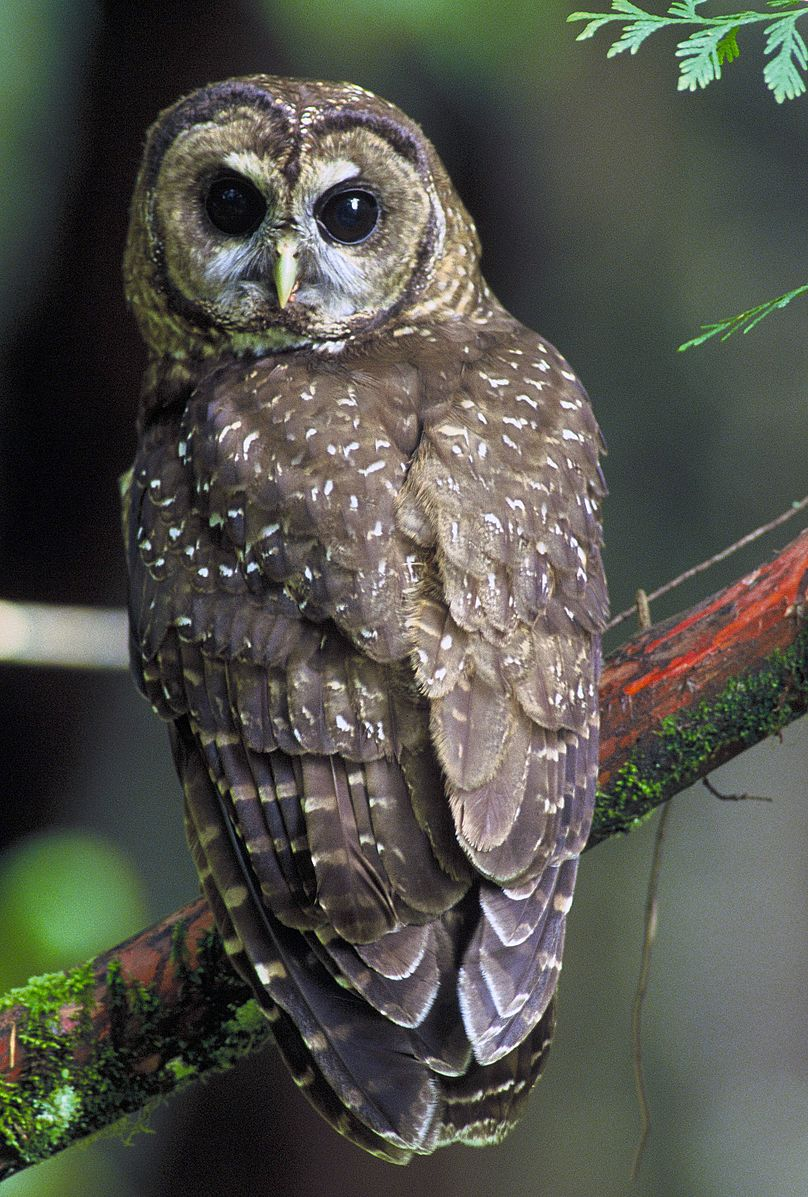
\includegraphics[width=.2\textwidth]{../images/NorthernSpottedOwl_USFWS}
\end{figure}

For these reasons, the managing entity, the United States Forest Service (USFS), would like to perform fuel removals in the Drink in order to reduce the area's fire hazard. However, while performing these fuel removals intends to provide long-term protection of the Drink Area, it has the potential to disrupt the habitat of the NSO \cite{bond2002short} and to induce short-term increases in sediment delivery \cite{o2005conceptual}. The latter is expected to be especially true in the Drink Area, where local USFS staff have noted that the watershed is unusually susceptible to spikes in sediment delivery as a result of foot traffic and other activities that occur within the watershed.

We developed a multi-objective mathematical program that optimizes the joint provision of these conflicting ecosystem services\footnote{These represent only a subset of the ecosystem services of concern to the USFS. While the USFS manages for many services simultaneously, many of the services are stacked rather than bundled, meaning the ecosystem services are not in conflict. These services need not all be considered in the multi-objective model, because the selection and maximization of one ecosystem service entails the maximization of all in the stack. For this reason, we have disregarded non-conflicting ecosystem services and selected a minimal bundle on which to employ multi-objective optimization. Those that do not conflict can be stacked post-optimization.}.

\subsubsection{The multi-objective model}
The multi-objective model is a zero-one mathematical program that assigns spatiotemporal prescriptions for fuel removals across the Drink Area to optimize the joint provision of ecosystem services. The spatial component of the prescriptions refers to the selection from the 303 forest stands into which the Drink has been divided (the interior polygons in Figure \ref{fig:drinkOverview}). Temporally, the model operates over an 80-year planning horizon, from 2015 to 2095. The fuel removals are scheduled in two 20-year treatment periods: 2015-2035 and 2035-2055. For each stand, the model may prescribe fuel removals in the first period, the second period, neither, or both.

The model minimizes the fire hazard rating of the Drink Area at the end of the 80-year planning horizon, maximizes the area of NSO habitat at the end of each planning period, and minimizes the short-term spikes in sediment delivery resulting from the application of silvicultural treatments. Furl removals are assumed to be performed at the midpoint year in the treatment periods: years 2025 and 2045 for the first and second periods, respectively. Figure \ref{fig:drinkPlanningHorizon} depicts the planning horizon of the study, showing the time of these events.

\begin{figure}
\centering
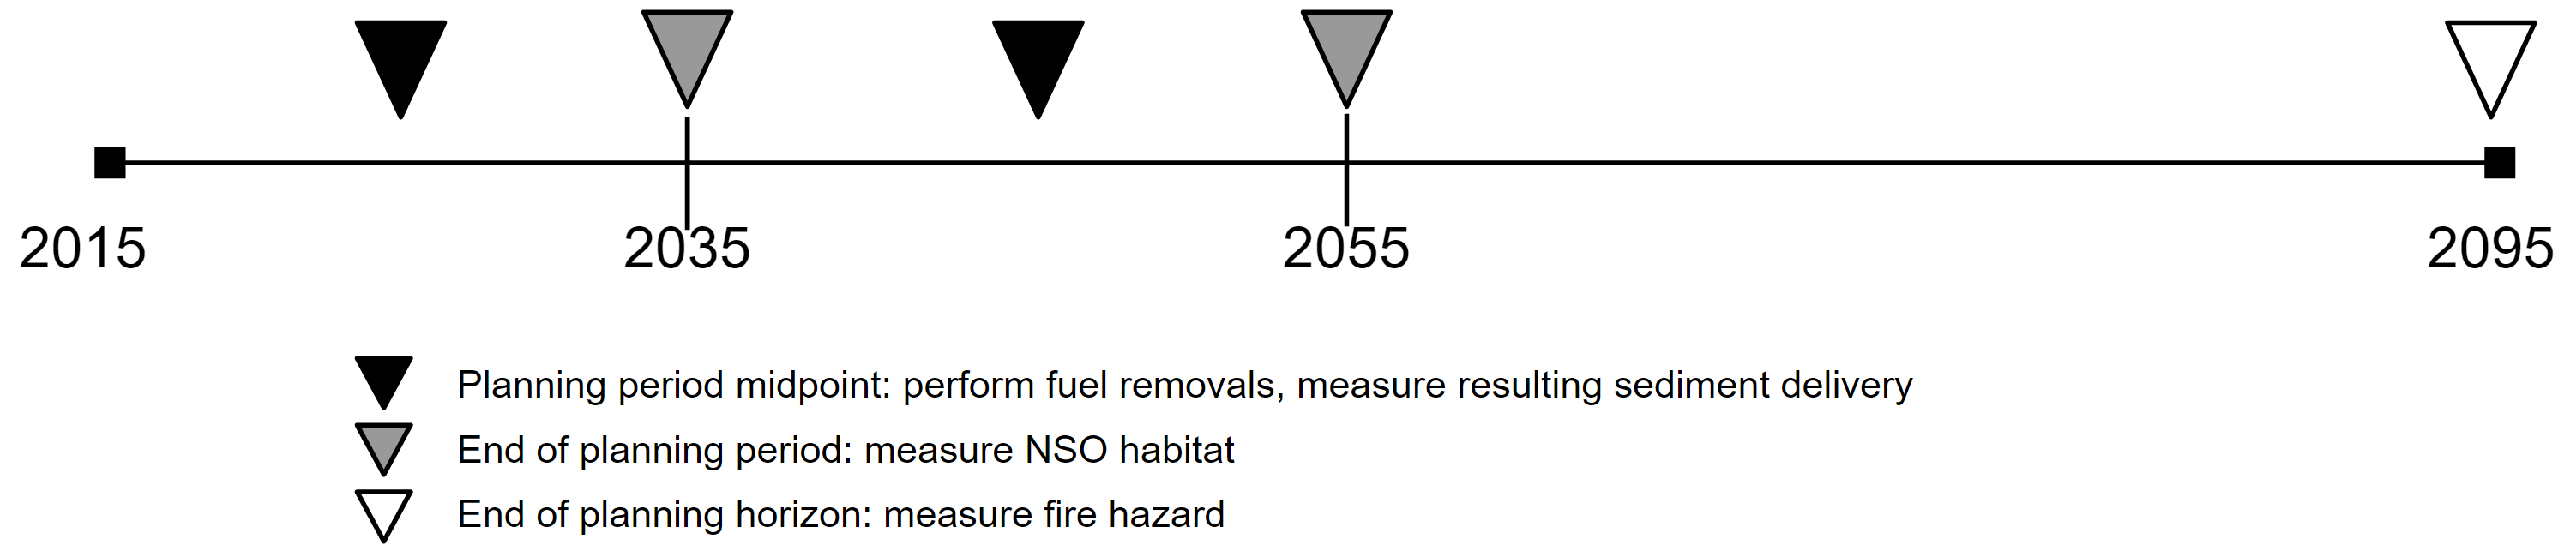
\includegraphics[width=.85\textwidth]{../images/Drink_PlanningHorizon_Sketch}
\caption[Planning horizon for the case study]{The planning horizon used in the case study spans the 80 year period from 2015 to 2095. Treatments may be performed in the first period, the second period, both, or neither. Treatments are assumed to be performed at the mid-point years of each period (black triangles). Sediment delivery is measured on treatment years. Stands' suitability for NSO habitat is measured at the end of the planning periods (gray triangles), and stands' fire hazard ratings are measured at the end of the planning horizon (white triangle).}
\label{fig:drinkPlanningHorizon}
\end{figure}

We use the following notation for the model.

\paragraph{Model parameters}
\begin{itemize}
\item \textbf{$i \in I$:} the set of forest stands comprising the Drink Area ($|I| = 303$)

\item \textbf{$a_i$:} the area of stand $i$

\item \textbf{$r \in R$:} the set of fuel removal prescriptions:
	$$
	r =
	\begin{cases}
	1 &\text{ treatment applied in the first period (2015-2035)}\\
	2 &\text{ treatment applied in the second period (2035-2055)}\\
	3 &\text{ treatment applied in both periods}\\
	0 &\text{ no treatment applied in either period}
	\end{cases}
	$$
	
\item \textbf{$F_{i,r}$:} the area-weighted fire hazard rating of stand $i$ at the end of the planning horizon if prescribed to fuel removal schedule $r$. The metric for fire hazard rating used in this analysis originated in the work by Schroder \textit{et al.} \cite{schroder2016multi}. This metric was developed for the Drink Area. It uses fire characteristics from the set of fuel models proposed by Anderson \cite{anderson1982aids} in order to assign a fire hazard rating. I expanded the rating system to include fuel models not present in Schroder \textit{et al.} See Table \ref{tab:firehazards}.

The USFS's Climate-Forest Vegetation Simulator (Climate-FVS) was used to generate the fuels and vegetation characteristics of the stands in order to determine their fire hazard rating. Initial vegetation data for Climate-FVS came from the 2012 GNN structure map (\url{http://lemma.forestry.oregonstate.edu/data/structure-maps}) from Oregon State University's Landscape Ecology, Modeling, Mapping \& Analysis (LEMMA) group. Plots from the LEMMA database were mapped to the stands in the Drink area in order to produce tree and stand lists. These lists were used with Climate-FVS to simulate the stands' vegetation and fuels characteristics forward for the duration of the planning horizon under each climate scenario. Input climate data for Climate-FVS was obtained through the Climate-FVS climate data server \cite{climateFVSReadyData}.

\begin{table}[!ht]
\centering
\resizebox{\textwidth}{!}{%
\begin{tabular}{l|c|crrr}
\multicolumn{1}{c|}{Fuel Model} & \multicolumn{1}{c|}{\textbf{Fire Hazard Rating}} & \multicolumn{1}{c}{Group} & \multicolumn{1}{c}{Flame length (m)} & \multicolumn{1}{c}{Rate of spread (m/hr)} & \multicolumn{1}{c}{Total fuel load (tons/ha)} \\ \hline
4*                              & \textbf{5}                                       & Shrub                     & 5.79                                 & 1508.76                                   & 32.12                                         \\
5                               & \textbf{4}                                       & Shrub                     & 1.22                                 & 362.10                                    & 8.65                                          \\
8                               & \textbf{1}                                       & Timber                    & 0.30                                 & 32.19                                     & 12.36                                         \\
9*                              & \textbf{2}                                       & Timber                    & 0.79                                 & 150.88                                    & 8.65                                          \\
10                              & \textbf{2}                                       & Timber                    & 1.46                                 & 158.92                                    & 29.65                                         \\
11*                             & \textbf{2}                                       & Logging Slash             & 1.07                                 & 120.7                                     & 28.42                                         \\
12                              & \textbf{4}                                       & Logging Slash             & 2.44                                 & 261.52                                    & 85.50                                         \\
13                              & \textbf{5}                                       & Logging Slash             & 3.20                                 & 271.58                                    & 143.57                                       
\end{tabular}%
}
\caption[Fire hazard ratings used in multi-objective model]{Fire hazard rating system used here, originally employed by Schroder \textit{et al.} \cite{schroder2016multi}.\\
Asterisks (*) denote fuel models not present in Schroder \textit{et al.}\\
The fuel model column refers to the Anderson fuel model ratings \cite{anderson1982aids}.}
\label{tab:firehazards}
\end{table}

\item \textbf{$I_{\omega,t}$:} the set of stands that qualify as NSO habitat at the end of planning period $t$ under at least one fuel removal schedule. The stands that qualify as NSO habitat at the end of a planning period $t$ are those that meet the following three criteria, as specified by the USFS:
	\begin{enumerate}
	\item elevation less than 1830 m
	\item the presence of trees with diameter at breast height (DBH) at least than 76 cm
	\item canopy closure of at least 60\%
	\end{enumerate}
The elevation requirement was checked using a digital elevation model from the US Department of Agriculture's GeoSpatial Data Gateway; canopy closure and large tree criteria were determined using the simulated vegetation characteristics output from Climate-FVS.

To account for the large habitat requirements of the NSO, stands must also be members of a cluster exceeding 200 ha in size, the entirety of which meets the aforementioned NSO habitat criteria. Stands that meet the first three criteria but are not part of such a cluster are less valuable NSO habitat and therefore have their contributions to the total owl habitat discounted by a factor of $e$.

\item \textbf{$e$:} the discount factor applied to NSO habitat when it is not part of a contiguous habitat cluster at least 200 ha in size. Following the convention used in Schroder \textit{et al.} \cite{schroder2016multi}, we set $e = 0.5$.

\item \textbf{$j \in R_{i,t}$:} the set of fuel removal schedules such that stand $i$ qualifies as NSO habitat at the end of planning period $t$. For instance, consider stand $i=15$ and planning period $t=2$ (2035-2055). We seek to find the set of fuel removal prescriptions $r \in R$ such that stand 15 is suitable NSO habitat at the end of planning period 2 (in year 2055). We enumerate the vegetation characteristics of stand 15 for all possible fuel removal schedules and determine that if fuel removals are assigned in the second planning period, then stand 15 does not qualify as NSO habitat in year 2055. Thus, $R_{15,2} = \{0,1\}$, since for $r=0$ (no fuel removals performed) and $r=1$ (fuel removals performed in first period only), stand 15 does qualify as NSO habitat in 2055.

\item \textbf{$s_{i,t}$:} the amount of sediment (in tons) delivered to the watershed as a result of performing fuel removals on stand $i$ in planning period $t$. The contributions of sediment delivery from treatment of stand $i$ in period $t$ were determined using the online GIS tool for the Watershed Erosion Prediction Project (WEPP) \cite{frankenberger2011development}. This tool takes soil textures, treatment types, duration of simulation, and custom climate data as inputs. Soil texture data for the Drink area was obtained from the USDA's Soil Survey Geographic (SSURGO) database, treatment types are those specified in \S \ref{chap:appendix_drinkTreatments}, and the years of simulation correspond to the treatment years in the planning horizon (2015-2095). The custom climate data are those described above for use with Climate-FVS, obtained through the Climate-FVS data server.

\item \textbf{$c \in C$:} Recall that the quantification of NSO habitat depends on the availability of large contiguous habitat patches; areas of NSO habitat less than than 200 ha in size are discounted. In order to determine when habitat is provided in sufficiently large areas, we must enumerate the set of clusters of stands whose combined area exceeds 200 ha. This set of clusters is the set $C$.

\item \textbf{$i \in D_c$:} Given a cluster $c \in C$, the set $D_c$ is the set of stands that comprise cluster $c$.

\item \textbf{$c \in C_i$:} Given a stand $i$, we define the set $C_i$ as the set of clusters that contain stand $i$

\item \textbf{$A$:} the maximum area in hectares that may be treated in either planning period. We constrain the allowable treatment area per period to account for the limited availability of work crews to perform the fuel removals. Following guidance from the USFS, we set $A = 2428$ ha (approximately 6000 ac).

\item \textbf{$\ell$, $u$:} the lower and upper bounds, respectively, on the relative fluctuation in the area treated in periods 1 and 2. These bounds are used to enforce regulation in the workflow for the USFS. Here we use values such that the area for which fuel removals are performed does not fluctuate more than 20\% between treatment periods; that is, we set the lower bound $\ell = 0.8$ and the upper bound $u = 1.2$.
\end{itemize}

\paragraph{Decision Variables}
$$
x_{i,r} = \begin{cases}
1 &\text{ if stand $i$ is prescribed to treatment schedule $r$}\\
0 &\text{ otherwise}
\end{cases}
$$ 

\paragraph{Indicator Variables}
\begin{itemize}
\item \textbf{$q_{c,t} = 1$} if all stands in cluster $c$ qualify as NSO habitat at the end of planning period $t$; $q_{c,t} = 0$ otherwise
\item \textbf{$p_{i,t} = 1$} if in planning period $t$ stand $i$ is part of a cluster $c$ such that $q_{c,t} = 1$; $p_{i,t} = 0$ otherwise
\end{itemize}

\paragraph{Accounting Variables}
\begin{itemize}
\item \textbf{$S_t$:} the total sediment delivered to the watershed from performing fuel treatments in planning period $t$
\item \textbf{$O_t$:} the amount of NSO habitat (in hectares) at the end of planning period $t$
\item \textbf{$H_t$:} the total area (in hectares) treated in planning period $t$
\end{itemize}

\subsubsection{Model formulation}
The formulation of the multi-objective model is as follows:
\begin{align}
Minimize \quad & \notag\\
&\sum_{i\in I}\sum_{r\in R} F_{i,r} x_{i,r} \label{eqn:objFire} \\
&\max \{S_1,S_2\} \label{eqn:objSediment} \\
Maximize \quad & \notag\\
&\min \{O_1,O_2\} \label{eqn:objOwl}
\end{align}
Subject to:
\begin{align}
\sum_{i\in I_{\omega,t}} \left(a_i p_{i,t} + e a_i \left( \sum_{j \in R_{i,t}} x_{i,j}-p_{i,t} \right) \right) &= O_t \qquad \forall t \in \{1,2\} \label{eqn:constraintDefOwl}\\
\sum_{i\in I} \sum_{r\in 1,3} s_{i,1} x_{i,r} &= S_1 \label{eqn:constraintSediment1} \\
\sum_{i\in I} \sum_{r\in 2,3} s_{i,2} x_{i,r} &= S_2 \label{eqn:constraintSediment2} \\
\sum_{i \in D_c} \sum_{j \in R_{i,t}} x_{i,j} - |c| q_{c,t} &\ge 0 \qquad \forall t \in \{1,2\}, c \in C \label{eqn:constraintClusterTriggers} \\
\sum_{c \in C_i} q_{c,t} - p_{i,t} &\ge 0 \qquad \forall t \in \{1,2\}, i \in I_{\omega,t} \label{eqn:constraintPVarTriggers} \\
\sum_{r \in R} x_{i,r} &= 1  \qquad \forall i \in I \label{eqn:constraintOnePrescrip} \\
\sum_{i \in I} \sum_{r \in 1,3} a_i x_{i,r} &= H_1 \label{eqn:constraintAreaAcctg1} \\
\sum_{i \in I} \sum_{r \in 2,3} a_i x_{i,r} &= H_2 \label{eqn:constraintAreaAcctg2} \\
H_t &\le A \qquad \forall t \in \{1,2\} \label{eqn:constraintAreaRestr} \\
\ell H_1 - H_2 &\le 0 \label{eqn:constraintAreaFlucL} \\
-u H_1 + H_2 &\le 0 \label{eqn:constraintAreaFlucU} \\
x_{i,r}, p_i, q_c \in \{0,1\} \quad &\forall i \in I, r \in R, c \in C \label{eqn:constraintNonNeg}
\end{align}

Equations \eqref{eqn:objFire}-\eqref{eqn:objOwl} are the objective functions: equation \eqref{eqn:objFire} minimizes the cumulative fire hazard rating of the Drink Area at the end of the 80-year planning horizon, equation \eqref{eqn:objSediment} minimizes the maximum peak in sediment delivery for the two planning periods, and equation \eqref{eqn:objOwl} maximizes the minimum NSO habitat available at the end of the planning periods. Equation set \eqref{eqn:constraintDefOwl} defines the amount of NSO habitat available at the end of the planning horizons. Note that if stand $i$ does not belong to a cluster of NSO habitat exceeding 200 hectares, then its area contribution to total NSO habitat is discounted by a factor of $e$. Equations \eqref{eqn:constraintSediment1} and \eqref{eqn:constraintSediment2} define the sediment delivered in planning periods one and two, respectively.

Inequality set \eqref{eqn:constraintClusterTriggers} controls the value of the cluster variables $q_{c,t}$ indicating clusters that meet the NSO habitat criteria in each of the planning periods. Inequality set \eqref{eqn:constraintPVarTriggers} controls the value of the $p_{i,t}$ variables indicating whether stand $i$ is included in a cluster of NSO habitat at time $t$.

The set of equalities \eqref{eqn:constraintOnePrescrip} enforces the logical constraint that each stand must be prescribed to exactly one fuel removal schedule. Equations \eqref{eqn:constraintAreaAcctg1} and \eqref{eqn:constraintAreaAcctg2} are accounting constraints for the total area treated in each planning period, and inequalities \eqref{eqn:constraintAreaRestr} ensure that this area does not exceed the predefined maximum. Inequalities \eqref{eqn:constraintAreaFlucL} and \eqref{eqn:constraintAreaFlucU} bound the fluctuation in treated area between the planning periods. Finally, constraint \eqref{eqn:constraintNonNeg} defines the decision and indicator variables as binary.

\subsubsection{Solution method}
We developed an implementation of T\'{o}th's Alpha-Delta algorithm \cite{TothThesis} to solve the model \eqref{eqn:objFire}-\eqref{eqn:constraintNonNeg} utilizing the IBM ILOG CPLEX optimization engine. For a problem with $M$ objectives, the Alpha-Delta algorithm finds the optimal set of solutions by iteratively slicing the $M$-dimensional objective space with a tilted $M-1$-dimensional hyperplane. The algorithm was implemented using an alpha parameter of $\alpha = .01$ and delta parameters of $\delta_{Hab} = 1$ ha and $\delta_{Sed} = 2$ tons for the NSO habitat and sediment delivery objectives, respectively.

\subsubsection{Climate change scenarios}
\label{sec:climateChange}
Like other ecosystems, forests will undergo changes as a result of the changing climate. For instance, researchers anticipate new spatial distributions of tree species \cite{iverson1998predicting}, increased sediment delivery to streams \cite{Goode20121}, and increasing disturbance regimes such as wildfires, droughts, and insect infestations \cite{vose2012effects}. As these transformations occur, the ability of forests to provide ecosystem services will change. Many studies have addressed the effects of climate change on isolated ecosystem services \cite{vose2012effects}\cite{bonan2008forests}\cite{mckenzie2004climatic}. However, forests provide these ecosystem services in concert with one another, and little attention has been given to understanding how climate change may impact the joint provision of ecosystem services.

The extent of this impact will likely depend on the severity of the realized climate change. Thus, to understand the potential impacts, multiple climate change scenarios representing a range of severities should be considered. In our case study, we consider three climate scenarios: one scenario in which climate change is ignored, ``None''; one in which climate change is predicted to be mild, ``Ensemble RCP 4.5'' (or ``E45''); and one in which climate change is predicted to be severe, ``Ensemble RCP 8.5'' (or ``E85''). These scenarios differ in their assumptions for the additional energy per unit area that will be absorbed by the atmosphere, a value known as radiative forcing (RF). In general, larger values of RF correspond to more severe climate change.

A given value for radiative forcing does not map to a single prediction of climate change, because researchers may disagree in how the climate will respond to a given amount of RF. Indeed, for a given RF, numerous climate models exist. A common approach to handling the disagreement among the climate models is to use an ensemble of climate models that all assume the same RF. We adopt this approach here for our E85 and E45 scenarios.

Each of these scenarios corresponds to an ensemble of 17 climate models that originate from the Fifth Assessment (AR5) performed by the Intergovernmental Panel on Climate Change (IPCC). The selection and assembly of the 17 climate models used in these ensembles was conducted by Cookston (2016) and the Climate-FVS team \cite{ClimateModelsInFVSEnsemble}.

The other scenario, None, ignores any effects of climate change. While the number of studies incorporating climate change is increasing, this is still the assumption used for many modern studies such as Schroder \textit{et al}. (2013) \cite{schroder2016multi}. Because it has served as the basis for many past studies of ecosystem services, the None climate scenario serves as a control against which to compare the other two.

Changing the climate scenario changes the parameterization of the model: the vegetation, fuels, and sediment delivery data depend on climate. Thus, changing the climate scenario can affect the amount and location of NSO habitat, the effects of fuel removals on NSO habitat, the fire hazard of the Drink Area, the efficacy of the fuel removals in reducing fire hazard, and the sediment delivered as a result of fuel removals. The result is a change in the interaction between ecosystem services and in the extent of conflict among them.